\documentclass[conference]{IEEEtran}

\usepackage{graphicx}
\usepackage{subfig}
\usepackage{multirow}
\usepackage{multicol}
\usepackage{array}
\usepackage{amsmath}
%\usepackage[style=authoryear-icomp,maxbibnames=9,maxcitenames=2,uniquelist=false,backend=biber]{biblatex}
\newcommand{\nltable}[2][c]{%
  \begin{tabular}[#1]{@{}c@{}}#2\end{tabular}}
\newcommand{\wave}{\raise.17ex\hbox{$\scriptstyle\mathtt{\sim}$}}

\newcolumntype{C}[1]{>{\centering\let\newline\\\arraybackslash}m{#1}}

\begin{document}
\bstctlcite{IEEEexample:BSTcontrol}

\title{DeepSpotCloud: Leveraging Cross-Region GPU Spot Instances for Deep Learning}


\author{\IEEEauthorblockN{Kyungyong Lee}
\IEEEauthorblockA{Department of Computer Science\\
Kookmin University\\
Seoul, South Korea\\
leeky@kookmin.ac.kr}
\and
\IEEEauthorblockN{Myungjun Son}
\IEEEauthorblockA{Department of Computer Science\\
Kookmin University\\
Seoul, South Korea\\
smj8612@kookmin.ac.kr}
}

% make the title area
\maketitle

\begin{abstract}
Cloud computing resources that are equipped with GPU devices are widely used for applications that require extensive parallelism, such as deep learning. When the demand of cloud computing instance is low, the surplus of resources is provided at a lower price in the form of spot instance by AWS EC2. This paper proposes DeepSpotCloud that utilizes GPU-equipped spot instances to run deep learning tasks in a cost efficient and fault-tolerant way. Thorough analysis about spot instance price history logs reveals that GPU spot instances show more dynamic price change pattern than other general types of cloud computing resources. To deal with the price dynamicity of the GPU spot instance, DeepSpotCloud utilizes instances in different regions across continents as a single resource pool. This paper also proposes a task migration heuristic by utilizing a checkpointing mechanism of existing deep learning analysis platform to conduct fast task migration when a running spot instance is interrupted. Extensive experiments using real AWS services prove that the proposed task migration method is effective even in a WAN environment with limited network bandwidth. Comprehensive simulations by replaying AWS EC2 price history logs reveal that DeepSpotCloud can achieve 13\% more cost gain than a state-of-the-art interrupt-driven scheduling policy. The prototype of DeepSpotCloud is implemented using various cloud computing services provided by AWS to serve real deep learning tasks. 
\end{abstract}

\IEEEpeerreviewmaketitle



\section{Introduction}\label{sec:intro}
Deep learning is a field of machine learning that tries to uncover multiple layers of non-linear hidden features in order to build a hierarchy of features to mimic how humans' brain works to recognize an object. Recent advancement of compute capacity with extensive parallel execution and improvement in the efficient algorithms make deep learning to widen its application scenarios in various fields, such as speech recognition, computer vision, natural language processing, and recommendation systems. 

Due to the nature of underlying neural-net algorithm of deep learning, extracting multiple layers of hidden features requires huge amount of compute capacity, and Graphics Processing Unit (GPU) devices are widely used as they can provide extensive parallelism. Some leading cloud computing service vendors provide compute instances that have GPUs. For instance, Amazon Web Service (AWS) provides G2 instances that are equipped with GRID K520 NVidia GPU cards - 1536 cores and 4GB of on-board memory. 

In AWS, users can utilize surplus of computing resources at a lower price than a regular on-demand instance price by exploiting \emph{EC2 spot instance}. The price of EC2 spot instance is decided based on an auction mechanism of which the supply and demand of compute resources in a given time window are the primary factors~\cite{spot-instance-pricing-analysis}. Despite of lower price of spot instances, resource volatility limits their applications to systems that have an inherent fault-tolerant mechanism or checkpointing capability~\cite{see-spot-run,spot-instance-checkpointing}.

Spot instances can be used to run deep learning tasks with a lower cost of operation. It is widely believed that using spot instance results in significant cost gain even less than 10\% of the on-demand instance price~\cite{spot-instance-pricing-analysis}. However, different from other types of EC2 instances, GPU instances have a uniqueness that host devices have to be physically equipped with GPU devices. In order to present unique availability patterns of GPU-based spot instances, Figure~\ref{fig:number-interrupt-bw} presents the number of interrupts per day in the vertical axis. The horizontal axis shows different EC2 instance types. For each instance type shown in the x-axis, the number of interrupts per day is measured across different Availability Zones (AZs), and a box-whisker figure is created with values of the different AZs. To measure the number of interrupts, we set the bid price as on-demand instance price of corresponding type~\cite{not-bid-cloud}. In the figure, it is observed that the mean and median number of interrupts for the GPU spot instance are much higher than other types of instances. In addition, the availability of GPU spot instance is highly variable across different AZs; a broader span of minimum, quartile, and a maximum number of interrupts. Owing to the distinct characters of GPU-based spot instances, running deep learning analysis tasks on the spot instances requires extra attention and heuristics.

\begin{figure}
    \centering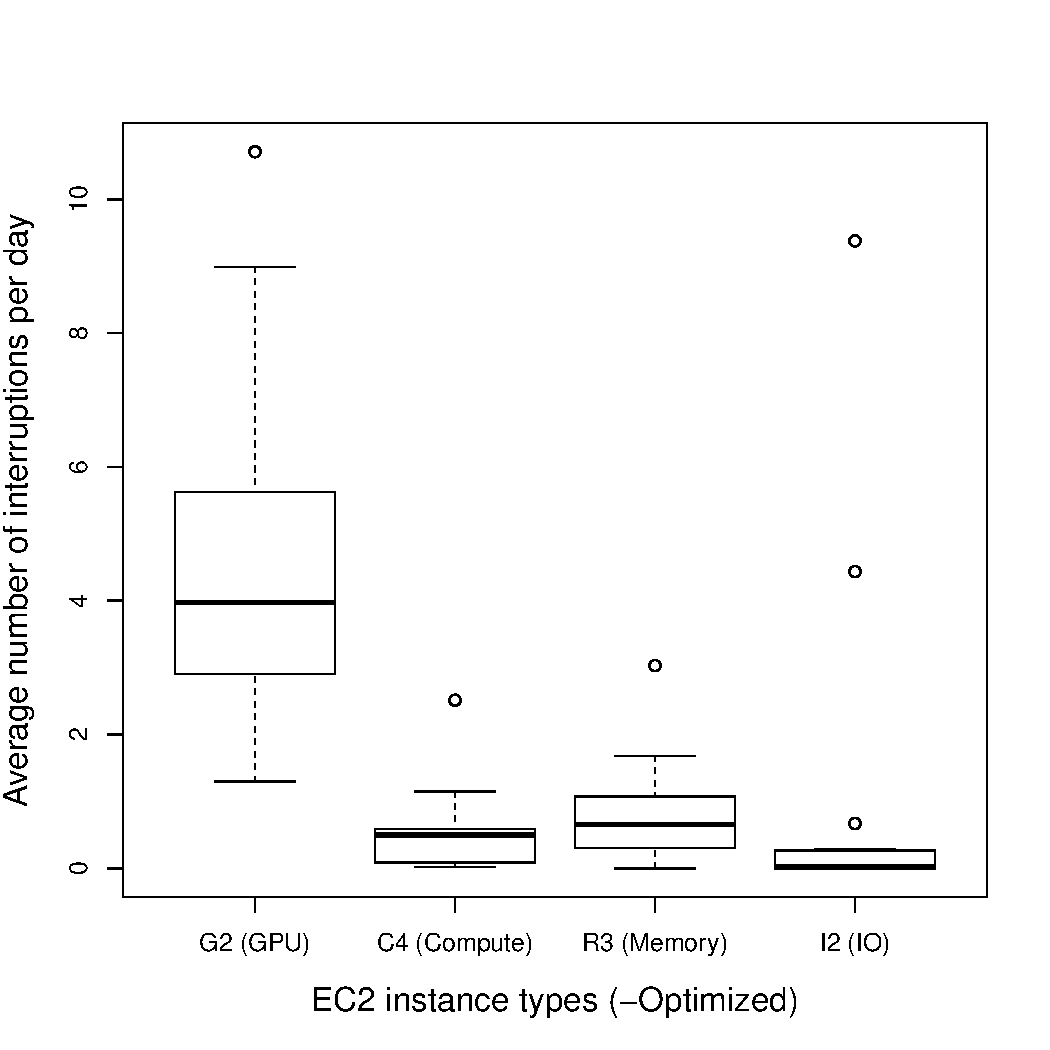
\includegraphics[width=0.4\textwidth]{figures/spot-instance-interrupt-bw.pdf}\caption{The number of interrupts per day for different EC2 instance types. The box whisker plot is created from metrics measured from different availability zones. GPU spot instances show a higher number of interrupts per day than other instances on average. GPU spot instances also show diversity in the number of interrupts across distinct AZs.\label{fig:number-interrupt-bw}}
\end{figure}

To execute deep learning tasks on GPU-based spot instances, fault-tolerant mechanisms of existing deep learning platforms must be revisited. Many of the existing deep learning platforms support checkpointing of intermediate result~\cite{tensorflow,mariana,poseidon}. Though checkpointing allows restarting a deep learning task from stored intermediate result, overall fault-tolerance mechanisms of deep learning platforms are limited comparing to other types of big data analysis platforms. For example, Hadoop~\cite{hadoop} and Spark~\cite{spark} provide extensive fault-tolerance mechanisms as they are intended to run on commodity hardware where failure is norm~\cite{google_mapreduce,late}. Using inherent mechanisms, Chohan et. al.~\cite{see-spot-run} and Flint~\cite{flint} proposed to use spot instances to run Hadoop and Spark tasks, respectively. 

Despite of uniqueness in the GPU-based spot instances and the limited inherent fault-tolerance mechanisms of existing deep learning platforms, there was no prior work that thoroughly investigates the opportunities and challenges of using GPU spot instances to run deep learning analysis tasks. To address the uniqueness of GPU spot instances, this paper first makes a comprehensive analysis about the availability pattern and cost gain of GPU spot instances comparing to other instance types. The analysis reveals that GPU spot instance has much higher degree of price diversity than others.

Based on the comprehensive analysis, this paper proposes DeepSpotCloud that exploits spot instances with GPU devices across different continents (regions) to perform deep learning analysis in a cost efficient way. Not being confined to resources within a single region, DeepSpotCloud utilizes a subset of instances across continents that are less expensive and expected to be more stable. To enhance fault-tolerance of the proposed system when a running spot instance is interrupted, we propose a novel architecture of lightweight task migration using a checkpointing feature of deep learning platforms in a WAN environment with limited network bandwidth. 

Extensive simulations are conducted to evaluate the cost gain and service availability of the proposed system by replaying the spot instance price logs provided by AWS. To present the applicability of the proposed system, DeepSpotCloud is implemented with AWS services and TensorFlow~\cite{tensorflow}. The implementation of DeepSpotCloud is executed on real-world GPU spot instances while running CIFAR-10 image classification tasks using convolutional neural network~\cite{cifar10}. The simulation result shows that the DeepSpotCloud can achieve 13\% more cost gain than a state-of-the-art interrupt-driven scheduling policy with only marginal additional overhead due to the task migrations. To the authors' best knowledge, this is the first work that proposes to utilize spot instances across different regions with sound engineering design to handle challenges that arise during the migration of workload across continents.

In summary, major contributions of this paper are as follow.
\begin{itemize}
    \item{Extensive analysis of GPU spot instance uniqueness}
    \item{Using GPU spot instances across different regions when running deep learning analysis tasks}
    \item{Proposing a lightweight deep learning task migration method in a WAN environment}
\end{itemize}

\section{Characterizing Spot Instance Price}\label{sec:character}
AWS EC2 offers various compute instances with distinct characters (Compute-, Memory-, IO-optimized, general, and GPU). To enhance service reliability, EC2 instance can be deployed in data centers that are physically separated. A \emph{region} in AWS is defined as a geographic area that is physically distant from others, such as America, Europe, and Asia. In the same region, multiple isolated data centers exist as \emph{Availability Zone (AZ)}. 

AWS provides its surplus of compute capacity at a lower price than that of on-demand or reserved instance type in the form of \emph{EC2 spot instance}. The price of spot instance is decided based on an auction mechanism where the supply and demand of compute resources are the primary factors~\cite{spot-instance-pricing-analysis}. To use it, a user bids for a spot price that one is willing to pay. If the bid price is higher than the current spot price of the requested type, a user has instances allocated and pays for the spot price (not the bid price) in an hourly rate. When an instance is running, if the bid price is outbid for a new spot instance price, the instance is terminated after two minutes of a grace period, and the output from the instance might be lost unless the outcome is stored in a storage. Using spot instance is known to be an economical way to utilize EC2 instances if applications can tolerate sudden service interruption.

\begin{figure*}
\centering
\caption{\label{spot-availability-heatmap}The ratio of spot instance price to that of on-demand instance. As the color becomes darker, the spot instance price becomes higher and closer to the on-demand instance price. GPU spot instances show darker color with more frequent changes.}
\begin{tabular}{ccc}
\multirow{2}{*}{
\subfloat[GPU Instances]{\label{spot-availability-heatmap-gpu}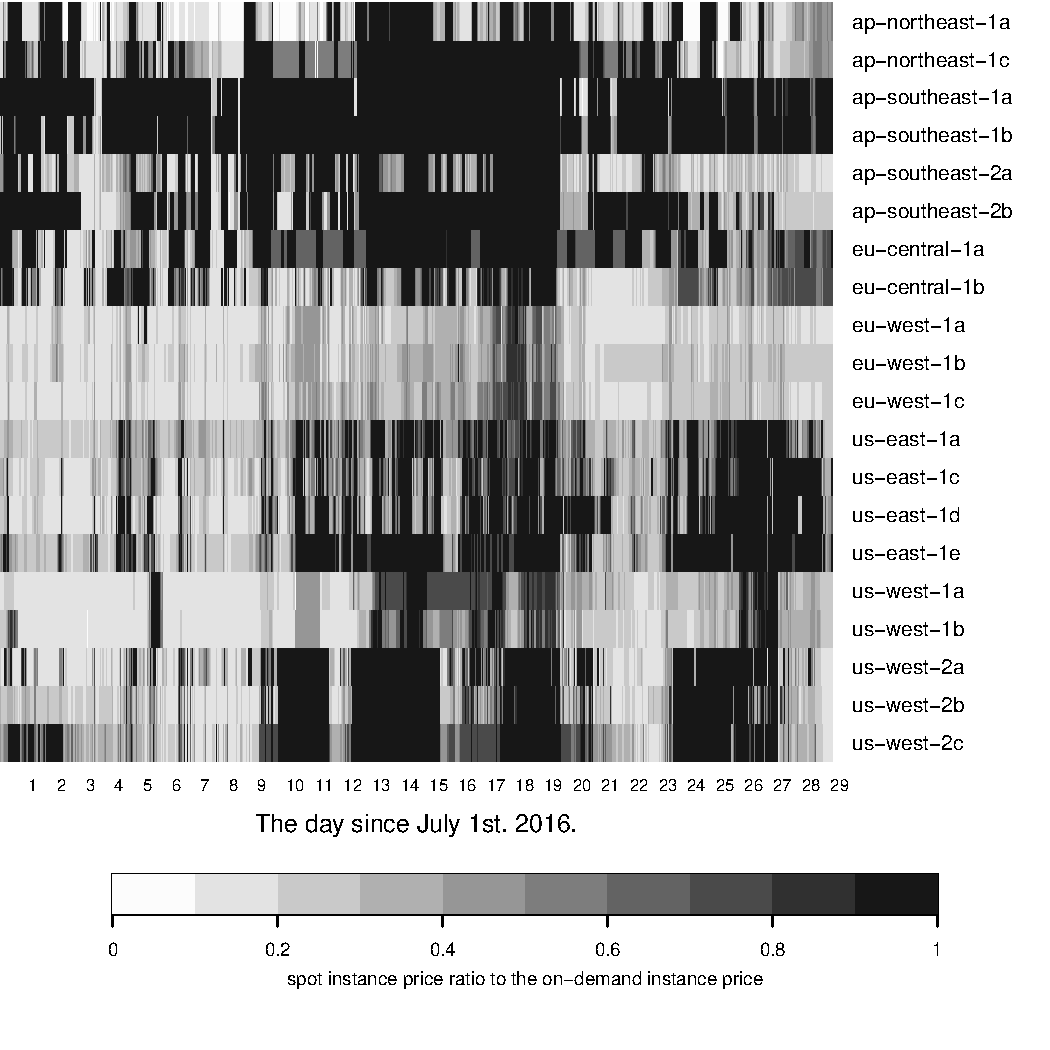
\includegraphics[width=0.47\textwidth]{figures/heatmap-g2-2x.pdf}}} &
\subfloat[Compute-optimized]{\label{spot-availability-heatmap-compute}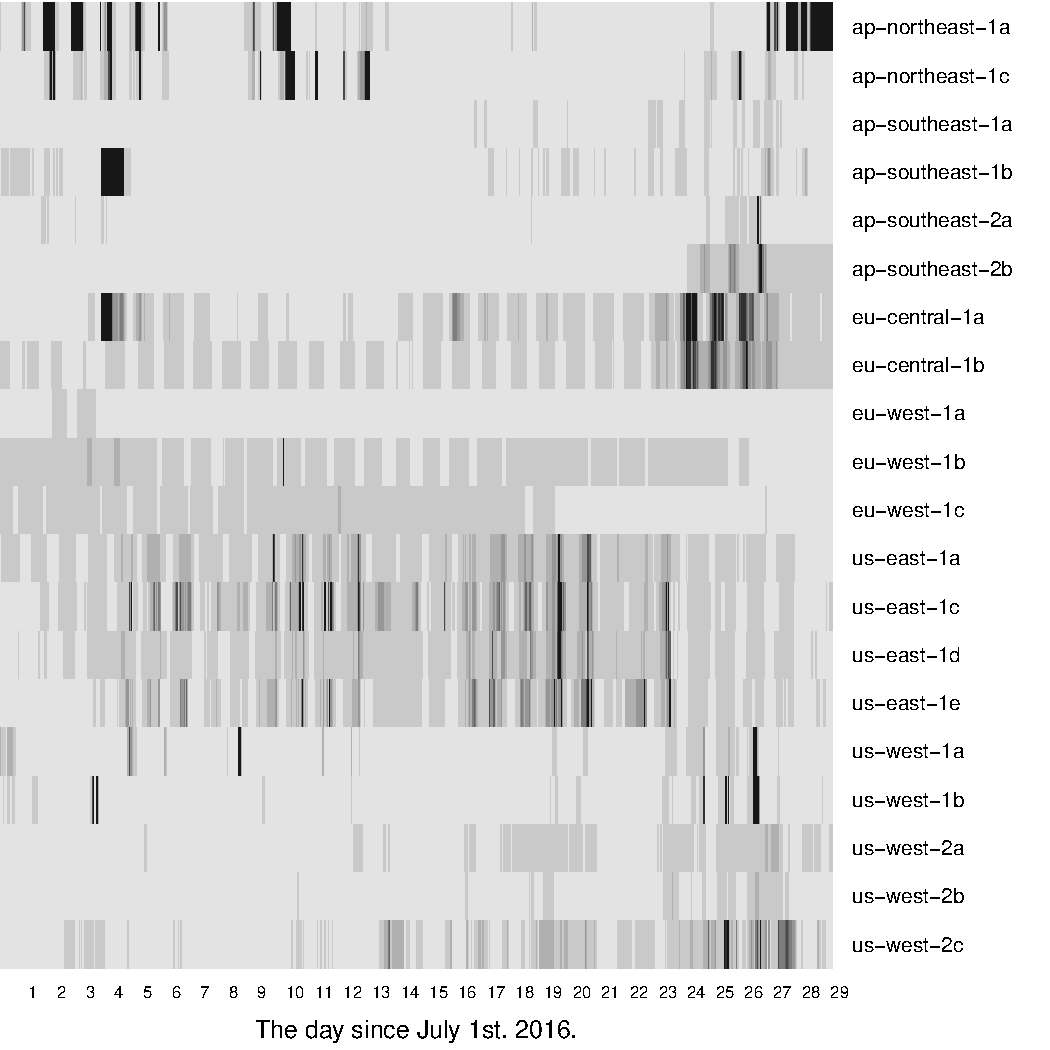
\includegraphics[width=0.2\textwidth]{figures/heatmap-c4-2x.pdf}} &
\subfloat[Memory-optimized]{\label{spot-availability-heatmap-memory}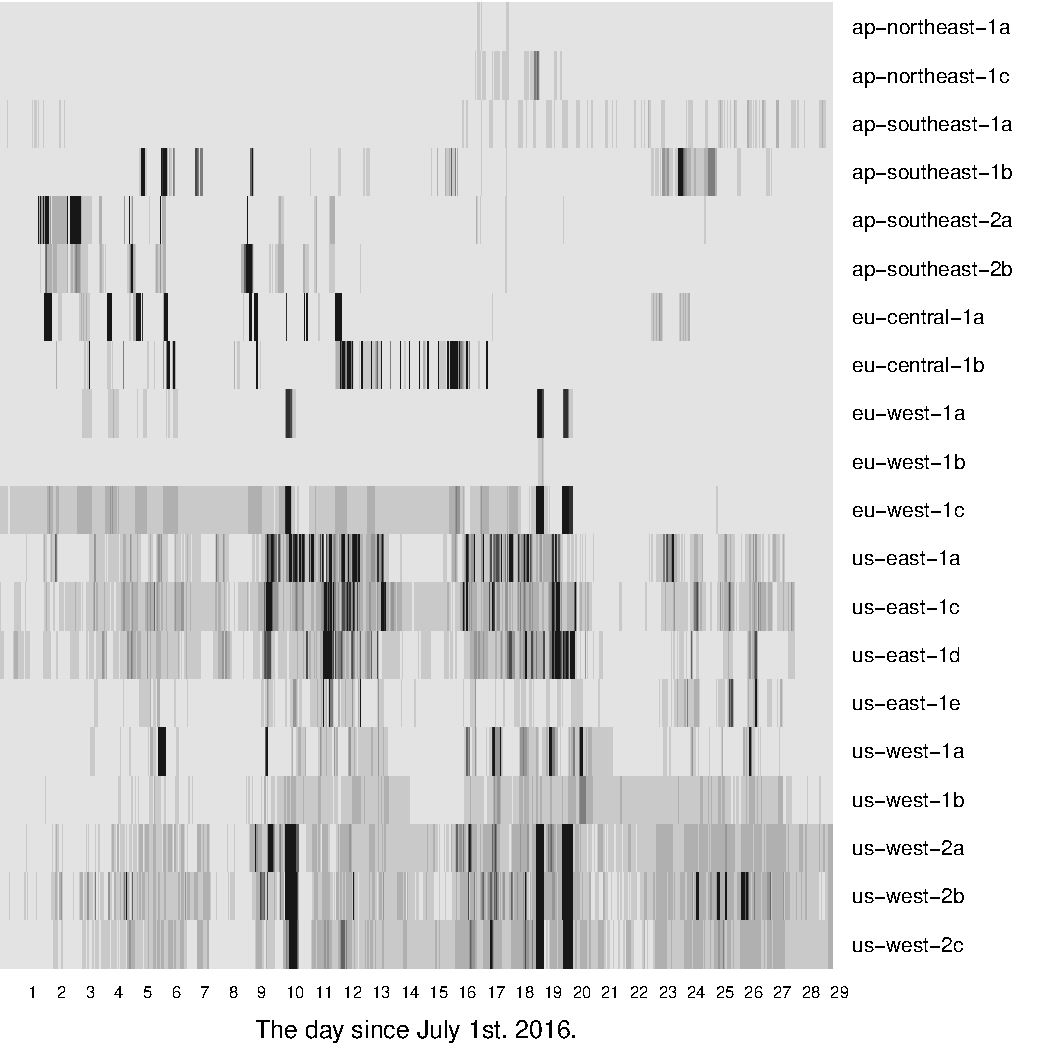
\includegraphics[width=0.2\textwidth]{figures/heatmap-r2-2x.pdf}}
\\
 & \subfloat[IO-optimized]{\label{spot-availability-heatmap-io}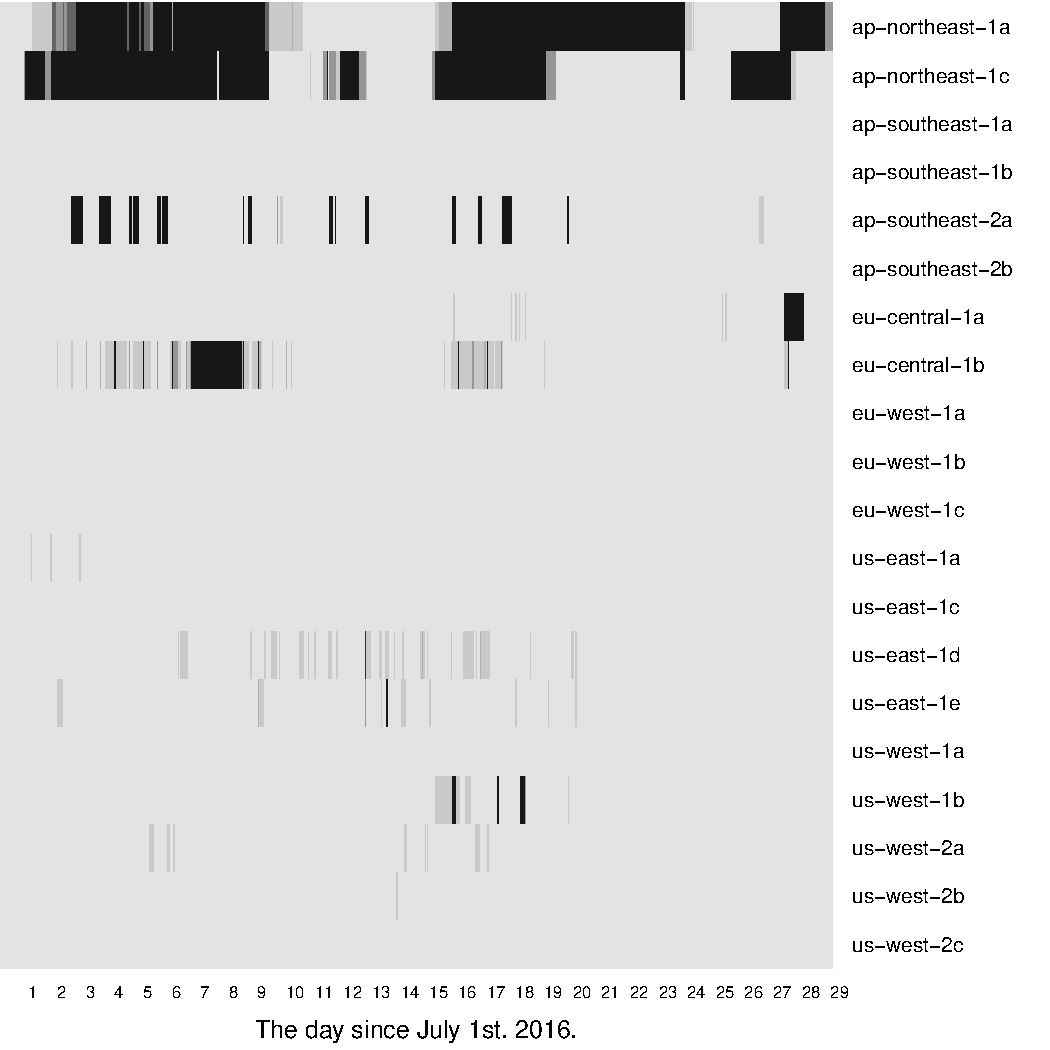
\includegraphics[width=0.2\textwidth]{figures/heatmap-i2-2x.pdf}}
& \subfloat[General-purpose]{\label{spot-availability-heatmap-general}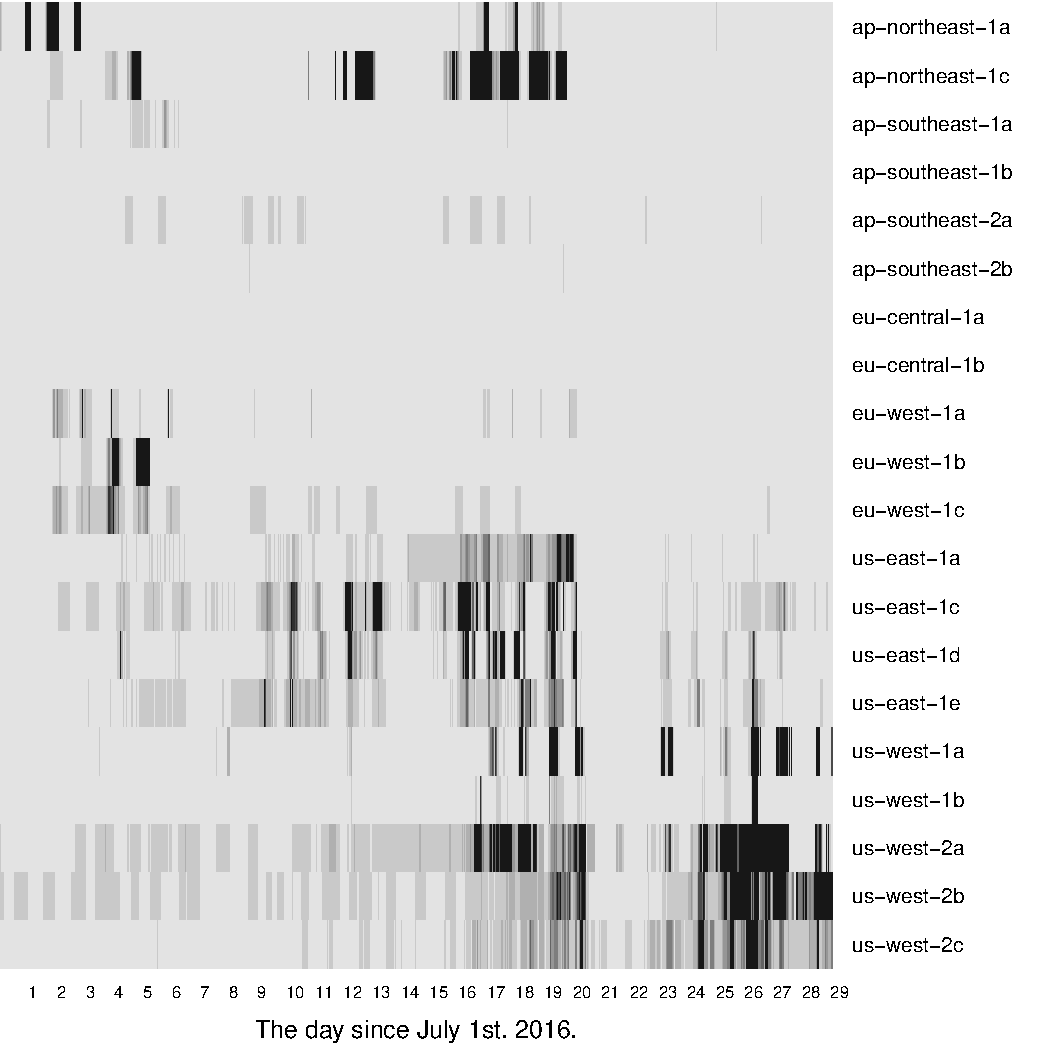
\includegraphics[width=0.2\textwidth]{figures/heatmap-m4-2x.pdf}}
\end{tabular}
\end{figure*}

\subsection{Uniqueness of GPU Spot Instance}
Among many EC2 instance types, GPU instance can provide extensive computing power for Single Instruction Multiple Data (SIMD) tasks by utilizing many cores in parallel on a GPU device, and deep learning platforms~\cite{tensorflow,caffe,theano} can benefit from the extensive parallelism as they generally require huge compute capacity.

\textbf{Price diversity of GPU-based spot instance}: GPU instances are also served in the form of spot instances in EC2, and people generally believe that using GPU spot instance would result in cost gain similar to that of other types of spot instances. However, different from others, GPU instances have a uniqueness that host devices have to be physically equipped with GPU devices - note that other types of instances (memory-, CPU-, and IO-optimized) are equipped with memory, CPU, and disk regardless of the type. Because of this trait, users might have a smaller pool of alternatives in choosing instances comparing to other types of instances. In order to present the distinctiveness of the GPU spot instance, Figure~\ref{spot-availability-heatmap} shows heatmaps that visualize the price ratio of EC2 spot instances to that of on-demand instances of different types. The ratio is calculated by the Equation~\ref{eq:price-ratio-spot-od}.
\begin{equation}\label{eq:price-ratio-spot-od}
  \text{Price Ratio = }\dfrac{Min(P_{si},~P_{od})}{P_{od}}
\end{equation}
$P_{od}$ and $P_{si}$ means the price of on-demand and spot instances, respectively, at the given time with the corresponding instance types. By taking the minimum of on-demand and spot instance price in the numerator, the ratio is capped at 1.0, and the ratio can reflect the cost that a user pays - note that there is no benefit of using spot instances by paying more than the on-demand instance price with the risk of unexpected interruption~\cite{not-bid-cloud}. In the figure, as the color becomes darker, the ratio gets closer to 1.0 (less cost gain). The lighter color means the ratio is closer to 0.0 (more cost gain). The ratio is calculated with AWS EC2 spot instance price history logs from July 1st. 2016, and the price is sampled at the every hour during the measurement period. The horizontal axis represents the elapsed days since the start time. The vertical axis shows AZs that provide corresponding instance types. The frequency of color darkness changes (light $\leftrightarrow$ dark) is the indication of the price change dynamicity - change across the horizontal direction can be interpreted as the \emph{temporal diversity} while the change in the vertical direction can be interpreted as the \emph{spatial diversity}. Figure~\ref{spot-availability-heatmap-gpu} shows the heatmap of GPU instance (\textit{g2.2xlarge}). For comparison, heatmaps of Compute (\textit{c4.2xlarge}), Memory (\textit{r3.2xlarge}), IO-optimized (\textit{i2.2xlarge}), and general purpose instance (\textit{m4.2xlarge}) are shown in Figures~\ref{spot-availability-heatmap-compute},~\ref{spot-availability-heatmap-memory},~\ref{spot-availability-heatmap-io}~\ref{spot-availability-heatmap-general}, respectively. As shown in the figures, spot instance price of GPU machines (Figure~\ref{spot-availability-heatmap-gpu}) has more darker spaces than others which means there is less cost gain when using GPU spot instances. In addition to the lower cost gain, GPU spot instance has more temporal and spatial price diversity than other instance types. 

To quantitatively evaluate the availability of spot instances, we calculate the ratio of time when the spot price is less than the on-demand price for various instance types. GPU spot instances show much lower availability; between May 4th and August 2nd, 2016, approximately 35\% of time, GPU spot instance price is higher than or equal to the on-demand price. Otherwise, general types of instances show much higher availability; the spot price is more expensive than on-demand price at most 5\% of the time. To better understand the cost gain of using spot instances, we calculate the cost that a user has to pay for different instance types. For GPU spot instances, users are expected to pay approximately 30\% of on-demand price. On the other hand, users of other instance types are expected to pay less than 20\% of corresponding on-demand instance price at most. Overall, the quantitative analysis result complies to the findings presented in Figure~\ref{spot-availability-heatmap}.
  
In summary, it is noticeable that GPU spot instances have lower availability and cost benefit comparing to other types of spot instances. Furthermore, availability and cost gain differ quite significantly across different AZs even in the same region. The findings in this section necessitate additional strategies to better utilize GPU spot instances in a stable and cost-efficient way especially for deep learning applications. 

\section{System Design}
As thoroughly analyzed in Section~\ref{sec:character}, GPU spot instances have uniqueness in the temporal and spatial price diversity with a limited set of instance types in a region. Furthermore, most deep learning analysis platforms support limited fault-tolerance features (model checkpointing) compared to other big-data analysis platforms. Considering such aspects, DeepSpotCloud, an orchestrator system enabling cost effective and fault-tolerant execution of deep learning applications on GPU spot instances, is proposed. It distinguishes itself from other systems~\cite{flint,spotcheck,see-spot-run} by utilizing GPU spot instances located globally across continents. There is a lower number of instance types that support GPU capability than other general instance types, and migrating tasks among GPU instances located globally would increase a pool of candidate resources to overcome the spatial diversity of price. By using globally located spot instances, however, a task migration across continents can cause significant overhead when a running instance is interrupted. In order to mitigate task migration overhead, DeepSpotCloud proposes a task migration method to decrease the data transfer overhead by using existing deep learning platforms' checkpointing mechanisms.

\subsection{Task Migration Heuristics: When to Migrate}
DeepSpotCloud categorizes task migration incidents into voluntary and forced migration. Voluntary migration happens at the service owner's willingness to decrease operation cost even when a service interruption event does not happen. Different from the voluntary migration, forced migration happens whenever an outbid event happens and a running instance is terminated within a short period of graceful shutdown time.

Voluntary migration has few options to decide when to initiate migration. First, \textbf{BestPrice} voluntary migration happens when the spot instance price of currently running AZ is more expensive than the lowest price AZ at the given time. This approach guarantees a task to run in an AZ where the spot instance price is lowest among all AZs. However, it can incur a significant number of task migrations if price changes frequently. Considering the overhead of task migration, initiating too many migrations can degrade overall performance.

The billing period of spot instance can also be considered to decide when to migrate a task voluntarily. Spot instance is charged hourly-basis as long as an instance is running. When an instance is terminated due to an outbid event, an instance is not charged for the partial hour till the time of interruption. However, when a user voluntarily shutdowns a running instance, the partial hour until the shutdown is charged as an hour. For example, if an instance runs for $h$ hour and $m$ minutes, a shutdown due to an interruption will incur $h$ hours of usage, while a voluntary termination will result in $h+1$ hours of usage. \textbf{BillingPolicy-Hourly} migration approach reflects the service providers' spot instance billing policy to avoid unexpected partial hour charge due to voluntary termination. He et al.~\cite{spot-server-migrate} proposed to reflect EC2 billing policy when making voluntary migration. However, different from DeepSpotCloud, the authors suggested to migrate an instance hourly whenever an interrupt event happens, and it is similar to the forced migration method in DeepSpotCloud.

\subsection{Task Migration Heuristics: How to Migrate}
Among many advantages of executing workloads on a virtualized environment, a live VM migration of running instances allows fast recovery from abnormal incidents. Similar to DeepSpotCloud, Kang et al.~\cite{live-migration-diaster} propose a middleware to perform live migration in a WAN environment of global-scale as a solution for a disaster recovery (e.g., earthquake). Though live migration helps to recover from some types of disasters that might allow about 10s of minutes of migration time, the shutdown preparation time of spot instance termination is only a few minutes that a live migration in a global-scale cannot complete. Xin et. al.~\cite{spot-server-migrate} claims that it is very challenging to complete a live VM migration even in the same region.

As the live migration cannot be a solution in global-scale, DeepSpotCloud utilizes existing deep learning platforms' checkpointing mechanisms. When a task migration is required, a checkpoint operation is initiated in a running instance. Most deep learning analysis platforms allow checkpointing intermediate outcomes per each iteration during modeling step, where an iteration is a unit of execution from a mini-batch of a large input dataset. In most GPU devices, one iteration can complete in a short time (at most few 100s of milliseconds). Considering per iteration time, it is reasonable to check necessity for checkpointing every iteration. After a checkpoint file is created, the outcome is uploaded to a permanent global storage to where a new spot instance has access. In parallel to checkpoint initiation, a new spot instance is started in an AZ that is predicted to be cost-beneficial. In the new instance initiation, a VM image that is equipped with all the necessary softwares is used to restart the task after fetching the checkpointed outcome from a storage.

\subsection{Task Migration Heuristics: Where to Migrate}
When a task migration happens either forced or voluntarily, choosing an AZ where a new instance is going to be launched is crucial to provide stable and cost-efficient operation. Previous research about analyzing AWS EC2 spot instance price~\cite{spot-instance-pricing-analysis} claims that the price change pattern of spot instances is rather random and it is challenging to predict future price based on the history of price change pattern. We confirmed the statement with GPU spot instances, and DeepSpotCloud deploys a new instance in an AZ where the current spot price is the lowest.

\subsection{System Architecture}\label{sec:architecture}
A high-level system architecture of DeepSpotCloud is presented in Figure~\ref{fig:architecture}. The core functions of DeepSpotCloud are implemented in the \textit{spot instance orchestrator} that performs tasks of spot price monitoring, instance recommendation, and instance arbitration. The spot price monitor periodically checks the current GPU spot instance price across all the AZs and keeps it locally to let an instance recommender reference. Instance arbitrator monitors the running spot instances to check if they are interrupted. In case a task migration is necessary, it prepares for task migration by initiating checkpointing operation and starting a new instance in an AZ based on the instance recommendation.

\begin{figure}
\centering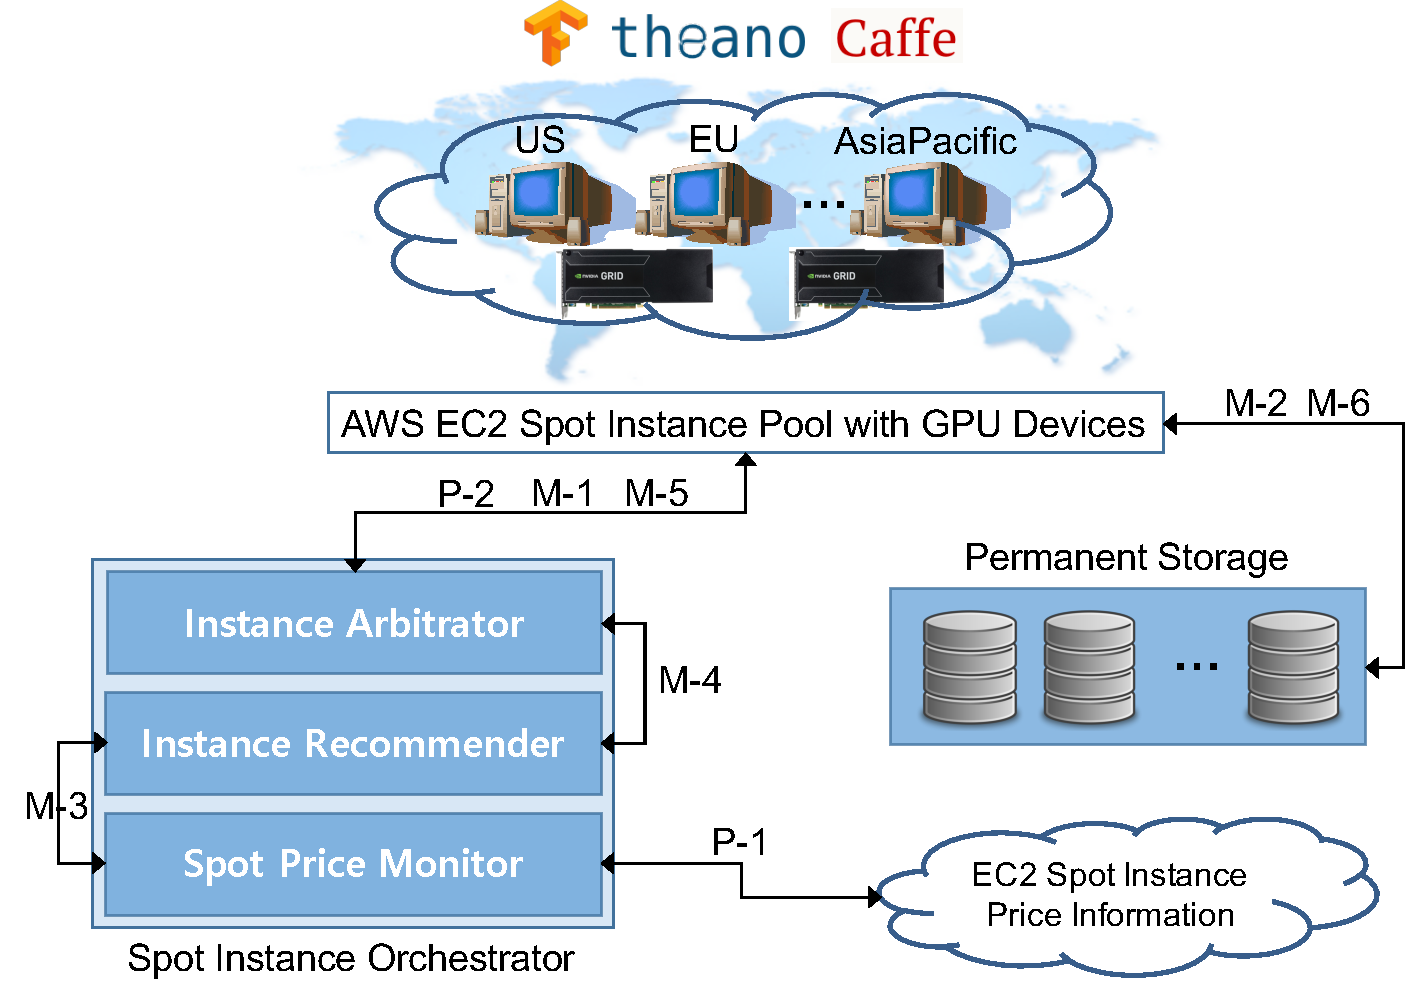
\includegraphics[width=0.42\textwidth]{figures/architecture.pdf}\caption{\label{fig:architecture}System architecture of DeepSpotCloud}
\end{figure}

In Figure~\ref{fig:architecture}, two types of operations are marked with \textit{P} and \textit{M} prefix, where \textit{P} means a periodic operation while \textit{M} notes an operation when a migration happens. \textbf{P-1} is an operation that spot price monitor periodically checks the current price of GPU spot instances and stores it locally. \textbf{P-2} is another periodic operation where the instance arbitrator checks if a running task needs to be migrated to other AZs.

As soon as a task migration becomes necessary (\textbf{M-1}), the arbitrator initiates a checkpoint operation to a running instance (\textbf{M-2}). The checkpointed outcome is uploaded to a global storage service so that a new spot instance can access the intermediate outcome. In parallel to checkpoint initiation, instance recommender makes suggestions about where to start a new instance by referencing spot instance price (\textbf{M-3}). As soon as the instance recommender notifies a suggested AZ (\textbf{M-4}), the arbitrator starts a new instance in the recommended AZ (\textbf{M-5}) with the checkpointed outcome path. As a new instance is launched, it fetches the checkpointed outcome from a shared storage (\textbf{M-6}) and restarts computation from the checkpoint.

\section{Implementation}\label{sec:implementation}
To present feasibility and applicability of DeepSpotCloud, a prototype is implemented using various AWS cloud computing services as shown in Figure~\ref{fig:implementation}. This section describes the details about the prototype implementation from the engineering perspective to ensure scalability and fault-tolerance of DeepSpotCloud. The current version of implementation is shared in GitHub\footnote{https://github.com/kmu-bigdata/deep-spot-cloud} with a demo web-page\footnote{http://bigdata.cs.kookmin.ac.kr/deep-spot-cloud-demo/}.

\subsection{Virtual Machine Image}
As shown in Figure~\ref{fig:implementation}, multiple spot instances run on globally distributed regions. To provide an identical execution environment, an Amazon Machine Image (AMI) is created in one region with Ubuntu 14.04, NVIDIA CUDA SDK 7.5, cuDNN library, and TensorFlow 0.1, and it is copied over to the distant regions using \emph{copy-image} feature by AWS.

\subsection{Spot Price Monitor}
Spot price monitor periodically communicates with the AWS API service to fetch the current spot instance price in all regions. In order to minimize implementation overhead of DeepSpotCloud, AWS Lambda service is used to check the GPU spot instance price. The function is triggered by Amazon CloudWatch, enabling it to run periodically every minute. The spot instance price is recorded to a permanent storage, DynamodDB, only when the price has been changed. The price history is referenced by \textit{instance recommender} to suggest an AZ to where a new instance is deployed. By storing the price history in a separate permanent storage service, scalability and fault-tolerance can be granted when the periodic price checker malfunctions or price inquiry requests spike.

\subsection{Instance Arbitrator}
Instance arbitrator is responsible for the orchestration of task migration. In order to decide whether a task migration is necessary, the instance arbitrator relies on the EC2 instance metadata~\cite{aws-metadata}. The spot instance termination notice is provided by the \textit{termination-time} metadata, and it can be accessed from a local HTTP web service. As soon as an instance detects a shutdown metadata, it sends a notification to the instance arbitrator with path information where a checkpoint outcome is uploaded to. The instance arbitrator utilizes Amazon API Gateway to receive an interruption notice from a spot instance. Upon getting an interruption notice, another AWS Lambda function is invoked to start a new spot instance in another AZ suggested by the \textit{instance recommender}.

When starting a new instance, the instance arbitrator passes a script to be executed after a new instance starts. Information about a deep learning task and the location of checkpointed outcome is passed via \emph{user-data}. The start script downloads the checkpointed outcome and starts a task written with TensorFlow continuing from the checkpoint. 

\subsection{Instance Recommender}
Instance recommender is responsible for suggesting an AZ where a new instance is going to be launched. Based on the previous work on predicting the price of spot instance, using advanced predictive analysis algorithms did not help to anticipate more stable and cost-efficient AZs~\cite{spot-instance-pricing-analysis}. Thus, the current version of DeepSpotCloud uses the current spot price to decide an AZ for a new instance. The dotted square box in the right bottom corner of Figure~\ref{fig:implementation} shows possible components for the instance recommender; AWS Kinesis for stream analysis and Amazon Machine Learning for advanced predictive analysis. Improving the accuracy of spot price prediction and building a system to perform the task is future work.

\begin{figure}
\centering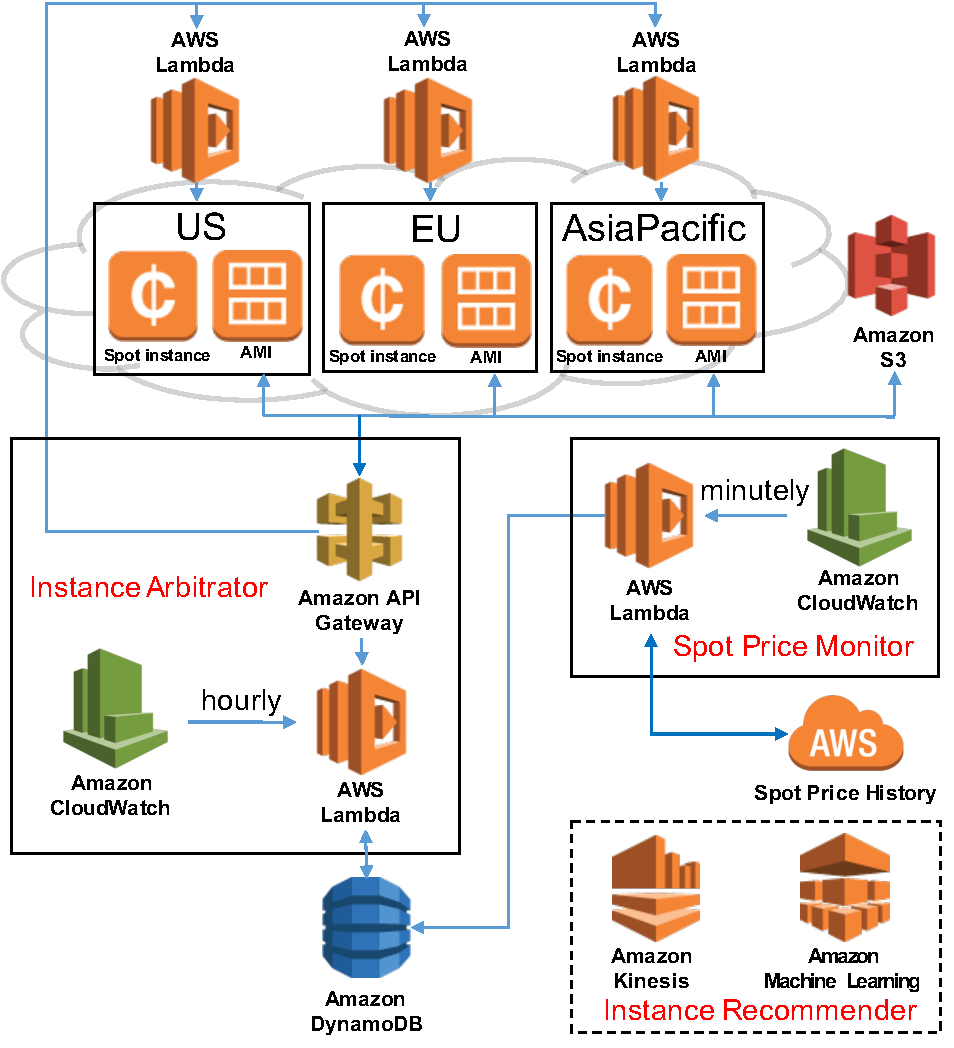
\includegraphics[width=0.45\textwidth]{figures/implementation.pdf}\caption{\label{fig:implementation}Implementation of DeepSpotCloud using various AWS services}
\end{figure}

\section{Evaluation}\label{sec:eval}
To analyze feasibility of the proposed task migration heuristics and the performance improvement from the methods in DeepSpotCloud, comprehensive simulations are conducted by replaying EC2 spot instance price history.

\subsection{Task Migration Overhead}
In the \textit{forced task migration}, a running spot instance has limited time to complete checkpointing; AWS EC2 allows two minutes before shutdown. In order to quantitatively analyze overhead from checkpointing and confirm whether the proposed mechanism can complete within the time window, task migration overhead is measured from the perspective of time to generate a checkpoint file and upload to a shared storage.

Figure~\ref{fig:checkpoint-time} shows the latency to create and store checkpoint files of different sizes. In the experiment, \textit{tf.train.Saver} class in TensorFlow~\cite{tensorflow} is utilized to generate a checkpoint file. The class provides \textit{save} and \textit{restore} method to create a checkpoint file and load the file to restart a session, respectively. In the figure, the vertical axis shows the latency, and the horizontal axis shows the checkpoint file size. The checkpoint file size ranges from 1MB to 1GB. The checkpoint file contains weight vectors whose dimension is dependent on the number of hidden layers, the number of neurons per each hidden layer, and the number of input/output neurons. In computation of forward and backward propagation, the entire weight vectors, input and output dataset of mini-batch size should be loaded into GPU device memory. In \textit{G2} family of EC2 instances, the equipped GPU card has 4GB of device memory. Considering the input and output dataset size, weight vectors whose size is larger than 1GB is not feasible to be handled in the \textit{G2} instance, and the experiment was conducted with up to the size. When storing a checkpoint file in an EC2 instance with EBS storage, one should be aware that the file system is connected through network, and the latency to store a checkpoint file can be prohibitive occasionally due to network instability. To deal with this issue, in the experiment, the checkpoint file is stored in the memory mapped file region (\emph{/dev/shm/}). Considering the checkpoint file size and criticality of checkpoint completion within a given time window, generating checkpoint file in a RAM disk region is a sound engineering choice. 

From the figure, it is observed that a task of storing checkpoint file completes within five seconds, and it does not pose a significant impact to complete a task migration within the graceful shutdown period. 
\begin{figure}
  \centering
  \caption{\label{fig:checkpoint-time}Time to generate checkpoint file of different size}
  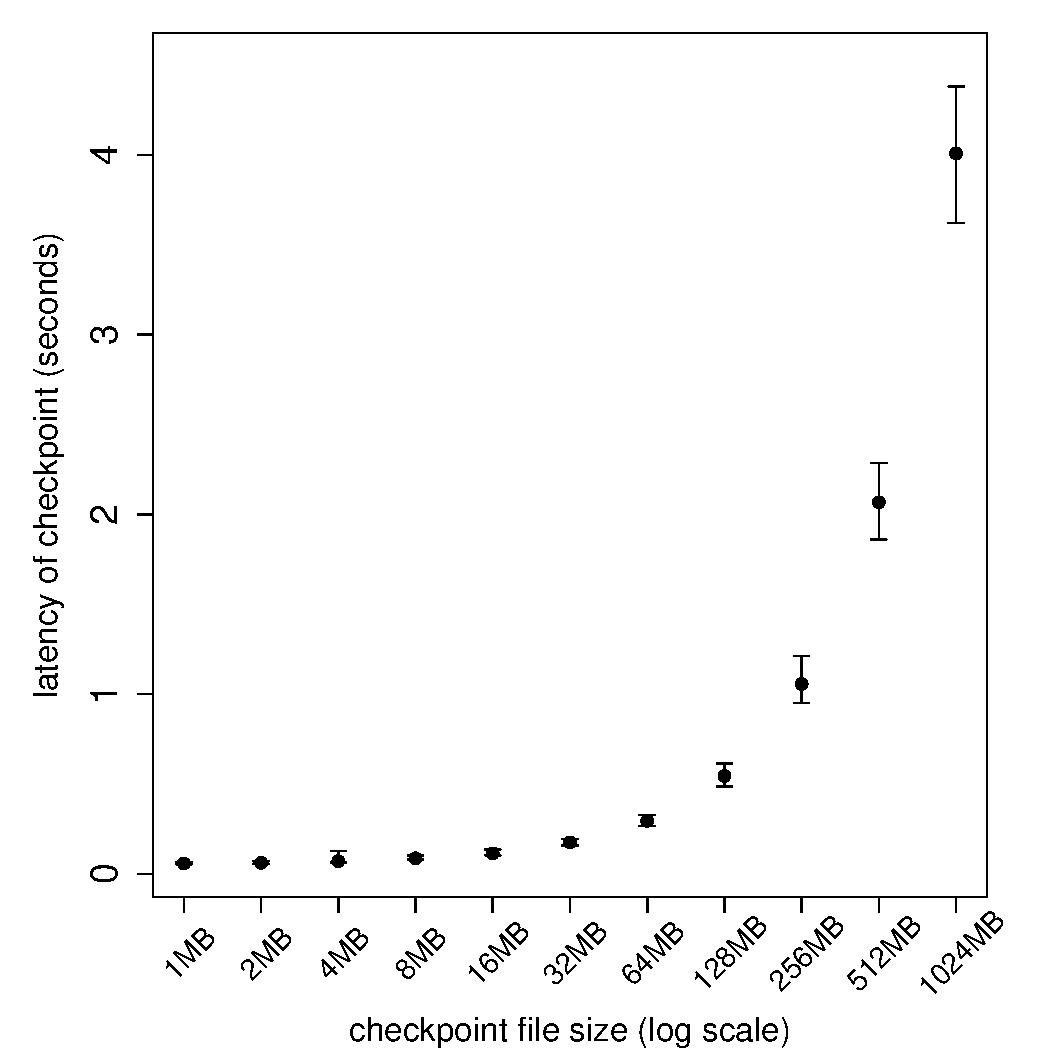
\includegraphics[width=0.35\textwidth]{figures/checkpoint-time.pdf}
\end{figure}

To complete a checkpoint process, the checkpointed file must be uploaded to a shared storage. DeepSpotCloud proposes to utilize AWS S3 as a shared storage service. When creating a S3 bucket, a user has to choose a region to locate a bucket. As the S3 bucket and DeepSpotCloud GPU spot instances can be located in any region, the checkpoint file upload latency is measured from all possible combinations of source and destination regions across continents with 1GB of checkpointed file. The average and maximum upload latency that is calculated after running each combination 100 times is shown in Table~\ref{table:cross-region-bw}. It is observed that uploading 1GB of checkpoint file takes in the order to 10s of seconds on average. The maximum latency was observed when uploading from Asia to US East region that takes 47 seconds. 

\begin{table}
\caption{\label{table:cross-region-bw}The latency to transfer between different regions}
\centering
\begin{tabular}{|C{0.8mm}| C{1.1cm}| C{1.3cm}|C{1.3cm}|C{1.3cm}|C{1.3cm}|}
\hline
\multicolumn{2}{|c|}{\multirow{2}{*}{}}&\multicolumn{4}{c|}{Destination}\\
\cline{3-6}
\multicolumn{2}{|c|}{}&US West & US East & Europe & Asia \\
\hline
\parbox[t]{2mm}{\multirow{4}{*}{\rotatebox[origin=c]{90}{Source}}}&US West& 11.9(22.5)& 20.4(37.7)&16.4(21.3)&13.3(15.5) \\
\cline{2-6}
&US East&14.4(24.7)&14.8(31.4)&12.9(14.4)&16.6(20.8) \\
\cline{2-6}
&Europe &18.1(24.7)&24.1(37.9)&10.0(10.8)&22.3(24.8) \\
\cline{2-6}
&Asia &13.8(16.2)&27.5(47.0)&21.0(10.8)&10.2(11.7) \\
\hline
\end{tabular}
\end{table}

Based on the experiments of checkpoint file creation and upload latency, two minutes of graceful shutdown period is enough to complete the checkpointing. Of 100 experiments, all the checkpointing operations complete within one minute even when a checkpointed weight vector is almost the maximum size that can be handled in the current \textit{G2} instances. 

\begin{table}
    \caption{\label{table:spot-instance-start-time}The time to start spot instances across regions (sec)}
\centering
\begin{tabular}{|C{1.5cm}|C{0.7cm}|C{0.8cm}|C{0.7cm}|C{0.7cm}|C{0.8cm}|C{0.7cm}|}
\hline
Metric&Min&$\frac{1}{4}$ Qu.&Median&Mean&$\frac{3}{4}$ Qu.&Max\\
\hline
Latency(secs)&86.5&96.5&110&121.6&126.6&242.9\\
\hline
\end{tabular}
\end{table}

A new spot instance start time is another factor that determines task migration overhead. In DeepSpotCloud, as soon as a task migration is scheduled, checkpointing intermediate result and a new instance initiation happen in parallel. As soon as both checkpointing and new instance initiation have completed, a migrated task resumes execution; thus, the total delay is dependent on the one that takes longer. Table~\ref{table:spot-instance-start-time} shows the distribution of latency to start a \textit{g2.2xlarge} spot instance in Europe, US East, US West, and Asia Pacific region. The instance initiation experiments are conducted 130 times with 10 minutes apart per each test. The time for new spot instance acquisition is measured from the spot request initiation to \textit{user-script} invocation time; \textit{user-script} is passed in a spot request and invoked after completion of instance booting. As shown in Table~\ref{table:spot-instance-start-time}, on average and 75\% of time, approximately two minutes are expected to take when starting a new GPU spot instance. From the overhead experiments, it is observed that the delay from task migration is mostly dependent on the new instance start time as both tasks are executed in parallel. 

\subsection{Migration Heuristics}
DeepSpotCloud proposes few heuristics when to migrate a task - forced migration when an outbid event happens (\textit{interrupt}), price-driven migration that always runs a task on the cheapest instance at the given time (\textit{best-price}), and billing policy-based migration that reflects billing policy of EC2 spot instance (\textit{hourly}). To evaluate each policy, we implement a simulator that replays EC2 spot price history of GPU instance (from May. 2016 to Nov. 2016). To mimic a realistic deep learning analysis tasks, we generate workloads that run for multiple iterations with different total running time (four hours, one day, three days, and one week). To realistically replay overhead from task migration, we used checkpoint latency and instance start time that is measured in a real EC2 environment. 1,000 simulations are conducted with randomly selected job start time and different total running time. The result is normalized to the value of \textit{interrupt} policy, a state-of-the-art task migration method utilized in He et al.~\cite{spot-server-migrate}

Figure~\ref{fig:migrate-cost} shows a normalized cost with different total running time. The \textit{best-price} policy incurs the most cost (five times more than the base policy). \textit{best-price} policy invokes a task migration whenever a region with the lowest price changes, and it incurs so many migrations that result in higher migration cost. Note that EC2 charges a fraction of hour usage (even few minutes) as a full hour in case of voluntary termination. Regarding \textit{hourly} policy, it saves approximately 13\% comparing to the base policy as the total task running time gets longer. The \textit{interrupt} policy makes the least number of task migrations only when necessary, and it does not have much impact on the overall cost when the task running time is short (four hours). However, as the total task running time gets longer, the impact of not using cheaper instance timely becomes noticeable.

Figure~\ref{fig:migrate-time} shows the normalized total running time with a base line policy of \textit{interrupt}. As a task migration happens, task execution is paused to create a checkpoint image and start a new spot instance. Though \textit{hourly} policy incurs more number of migrations than \textit{interrupt} policy and results in less cost (Figure~\ref{fig:migrate-cost}), the impact to the overall task running time is marginal; at most 1\% of total running time is increased.

The results present that the proposed voluntary task migration mechanism (\textit{BillingPolicy-Hourly}) achieves noticeable cost gain while incurring only marginal additional task running time. Cost savings of DeepSpotCloud comparing with that of on-demand instances from real-world deployment can be found on a demo website.

\begin{figure}
  \centering
  \caption{\label{fig:migraion-evaluation}Evaluation of task migration policy}
  \subfloat[normalized price consumption]{\label{fig:migrate-cost}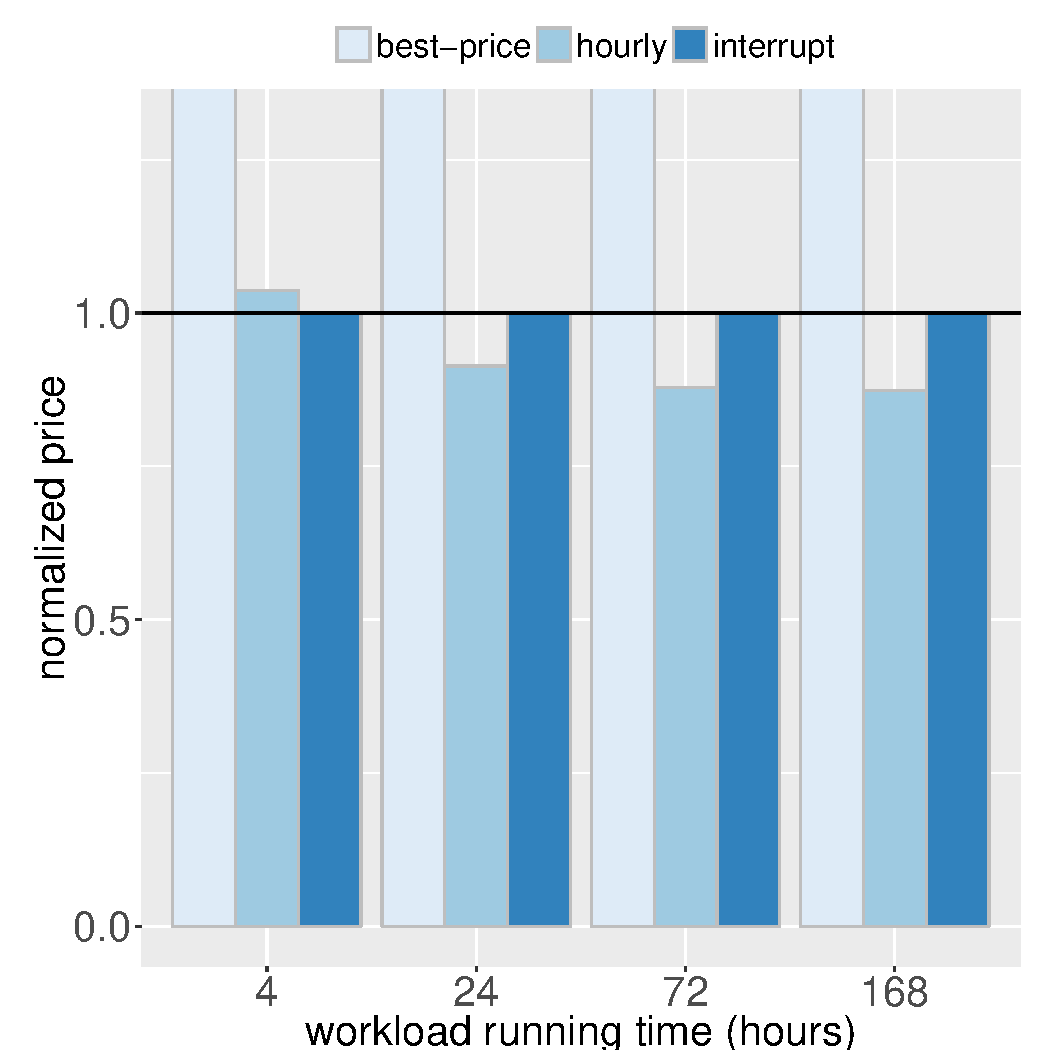
\includegraphics[width=0.25\textwidth]{figures/migration-plan-price-compare.pdf}}
  \subfloat[normalized task completion time]{\label{fig:migrate-time}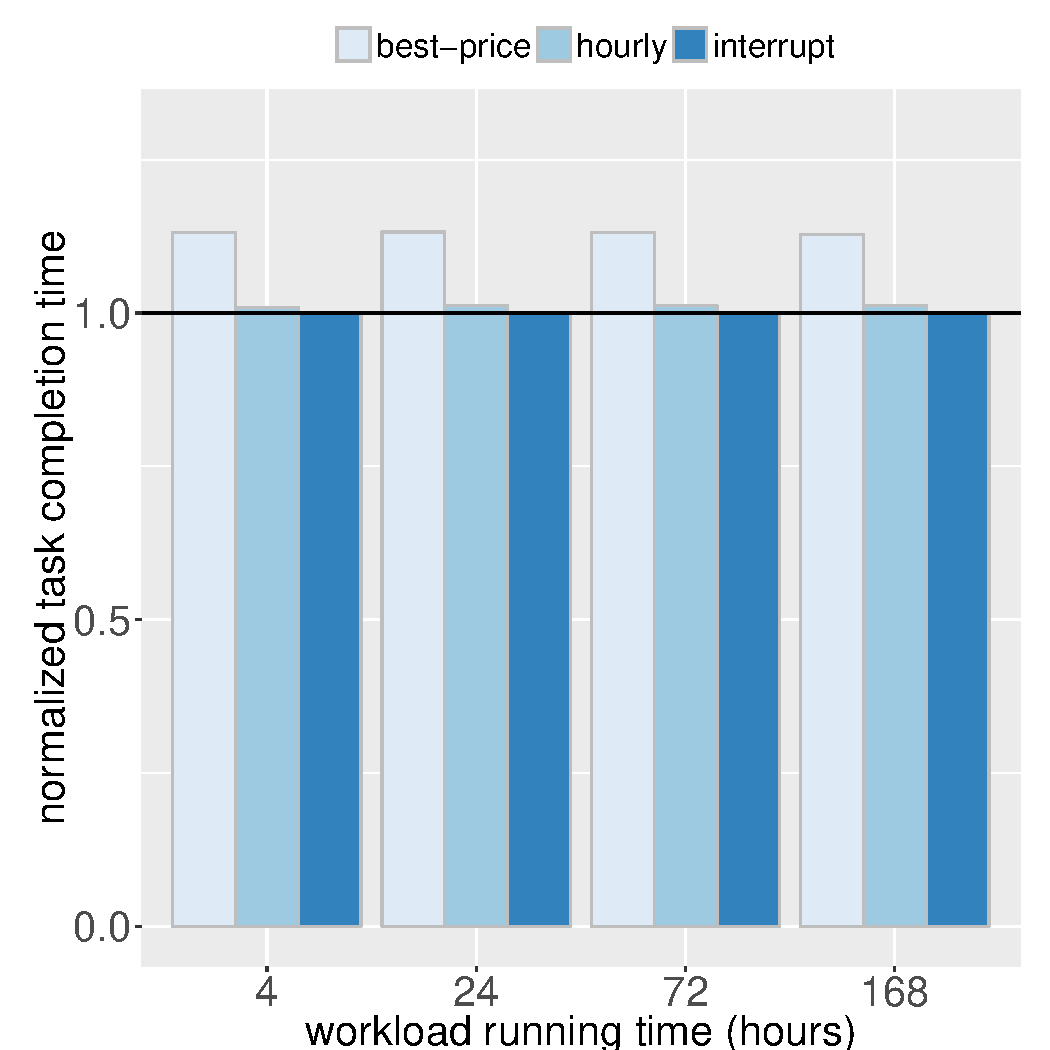
\includegraphics[width=0.25\textwidth]{figures/migration-plan-latency-compare.pdf}}
\end{figure}

\section{Related Work}
In the context of using spot instances for big-data processing, SeeSpotRun~\cite{see-spot-run}, Flint~\cite{flint}, and TR-Spark~\cite{tr-spark} propose to run Hadoop or Spark on spot instances. They focus on heuristics of handling an unexpected interruption due to an outbid event. The mechanisms proposed in the research utilize inherent fault-tolerance mechanisms of Hadoop and Spark (automatic task re-execution and RDD lineage) that are not supported by most deep learning platforms. SpotCheck~\cite{spotcheck} and He et al.~\cite{spot-server-migrate} propose to utilize various types of spot instances as a single derivative resource pool. They propose a fast VM migration method to deal with an outbid event. The proposed methods target general types of instances on a same region. As discussed in this paper, GPU spot instances have unique characters with respect to the availability and price change pattern, and the proposed methods are not directly applicable to GPU spot instances. The authors also claim that using spot instances across regions is challenging and remaining work. Characteristics of spot instances are well studied in literature Zheng et al.~\cite{how-to-bid-cloud}, Sharma et al.~\cite{not-bid-cloud}, Javadi et al.~\cite{si-price-modeling}, and Ben-Yehuda et al.~\cite{spot-instance-pricing-analysis}. They focused on analyzing all types of spot instances but could not uncover uniqueness of GPU spot instances.

\section{Conclusion and Future Work}
This paper presents DeepSpotCloud, a novel approach to utilize GPU spot instances in a cost efficient way to execute deep learning workloads. Based on thorough analysis about spot instance price of various types, we discovered that GPU spot instances have uniqueness in the price change pattern - temporal and spatial diversity. To deal with the diversity and a limited number of GPU instances, DeepSpotCloud proposes to use GPU spot instances across continents. This paper also presents a task migration method when a spot instance is interrupted. Evaluation of the proposed task migration method using real AWS cloud computing services confirms that two minutes of shutdown preparation time is enough to complete a task migration even in a WAN environment. Extensive simulations conducted by replaying EC2 spot instance price history logs reveal that a proposed \textit{BillingPolicy-Hourly} migration heuristic achieves 13\% cost gain while incurring marginal task migration overhead. The prototype of DeepSpotCloud is implemented using various AWS cloud computing services and shared in GitHub.

DeepSpotCloud currently uses only the most recent price to select the optimal AZ to deploy a new instance. Advanced predictive analysis can be applied to predict more cost efficient and stable AZs. The current version of DeepSpotCloud supports a deep learning task that runs on a single GPU instance, and we are working on applying DeepSpotCloud on a distributed deep learning analysis platforms with multiple workers in distinct regions that utilize a parameter server~\cite{parameter-server}. In such scenario, task migration heuristics need to be further improved to handle a task with larger model size. 

%The current DeepSpotCloud executes deep learning tasks only on GPU-based spot instances, but when considering other factors in task migration such as cost, availability, and scalability, choosing other GPU spot instances besides g2.2xlarge spot instance or non-GPU spot instance as the migration destination may be feasible. analyzing the impact of resource heterogeneity to the overall performance is an interesting topic for future work. In addition, we are working on using other deep learning algorithms and frameworks besides convolutional deep neural network and Tensorflow.

\section*{Acknowledgment}
We would like to thank anonymous reviewers for their insightful comments and Dongeon Kim to help building a demonstration website. This work is supported by the National Research Foundation of Korea (NRF) Grant funded by the Korean Government (MSIP) (No. NRF-2015R1A5A7037615 and NRF-2016R1C1B2015135), the ICT R\&D program of IITP (2017-0-00396), the AWS Cloud Credits for Research program.

% trigger a \newpage just before the given reference
% number - used to balance the columns on the last page
% adjust value as needed - may need to be readjusted if
% the document is modified later
%\IEEEtriggeratref{8}
% The "triggered" command can be changed if desired:
%\IEEEtriggercmd{\enlargethispage{-5in}}

% references section

% can use a bibliography generated by BibTeX as a .bbl file
% BibTeX documentation can be easily obtained at:
% http://mirror.ctan.org/biblio/bibtex/contrib/doc/
% The IEEEtran BibTeX style support page is at:
% http://www.michaelshell.org/tex/ieeetran/bibtex/
\bibliographystyle{IEEEtranS}
\bibliography{deep-spot-cloud}
\end{document}


